Does weighting the comparison to the common support remove false alarms without suppressing power for genuine harmful change? We compare six modes representing three weighting families: unweighted (no correction), Crump trimming (hard threshold at $\min(p,1-p) \geq 0.1$), overlap weights (continuous propensity-score weighting via $p(1-p)$), and stabilized density-ratio weighting (source-weighted, target-weighted, and doubly weighted). All six modes share the same one-sided permutation test (D-SOS); only the weights differ. Crump and overlap weights come from the causal-inference literature~\cite{Crump_2009, Li_2018_balancing}; both address overlap, but neither incorporates the asymmetric density-ratio corrections that handle two-sided mismatch. A comprehensive comparison of the three weighting families is provided in Appendix Table~\ref{tab:weighting-benchmarks}.

\subsection{False Alarms from Weak Overlap}\label{sec:calibration}

In the null scenario, source and target behave identically on the common support, but weak-overlap regions on both sides have different score distributions. The unweighted test over-rejects as weak overlap increases (Figure~\ref{fig:calibration}). Source-weighted and target-weighted modes also over-reject because each corrects only one side. The doubly weighted test stays at or below the 5\% nominal level across the entire severity grid (Table~\ref{tab:calibration-reject}). A second synthetic DGP with 2D features and a linear score function reproduces this pattern (Appendix~\ref{app:second-dgp}).

The two causal-inference baselines reveal the structural weakness of weighting the propensity score rather than the density ratio (Table~\ref{tab:weighting-benchmarks}). Crump trimming drops observations with $\min(e,1-e) < 0.1$ and runs an unweighted test on the remainder; it over-rejects because the remaining sample still carries two-sided mismatch. Overlap weights assign continuous weight $w(x) = e(x)(1-e(x))$, which downweights extreme propensities smoothly. But the weight is symmetric---it treats both groups identically---and cannot correct asymmetric two-sided contamination. Stabilized RIW differs in two respects: it weights the density ratio rather than the propensity score, so the prior ratio and group-conditional densities shift the weight shape; and its forward/inverse corrections handle each group's density structure separately. Only the doubly weighted mode---both corrections active simultaneously---resolves two-sided mismatch.

A notable asymmetry appears at low severity: source-weighted rejects at 43\% and target-weighted at 6\% at severity 0.1. This follows from the DGP structure---weak-overlap mass is symmetric, but the source distribution (a standard Gaussian) has heavier tails in the target-specific region than the target mixture has in the source-specific region, so the target weight correction is more aggressive. The asymmetry reverses at higher severity as both sides saturate. Only the doubly weighted test resolves two-sided mismatch regardless of which side dominates the weight correction.

The stabilization parameter $\lambda$ controls this trade-off explicitly: at $\lambda = 0.75$ the doubly weighted test over-rejects ($66\%$ false alarm at severity $0.25$), approaching unweighted behavior as $\lambda \to 1$; $\lambda = 0.25$ maintains calibration ($0\%$) through stricter common-support restriction. Appendix~\ref{app:lambda} reports the full grid.

\begin{figure}[t]
	\centering
	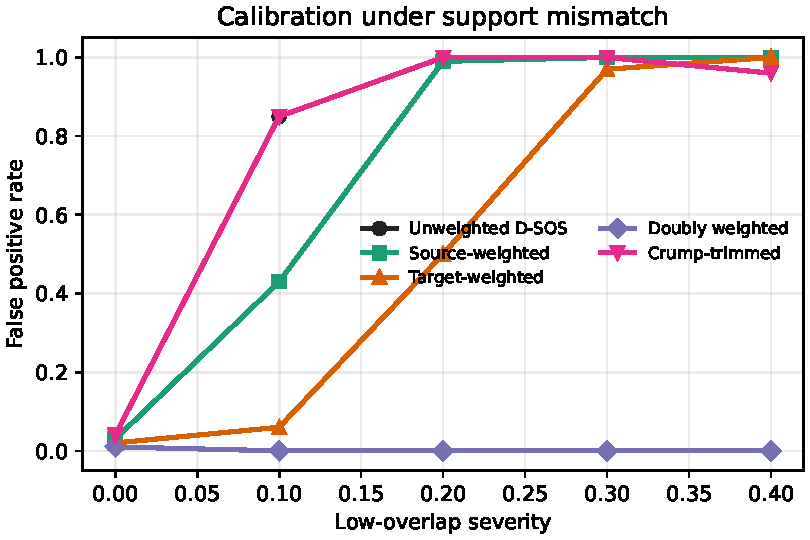
\includegraphics[width=0.95\linewidth]{figures/calibration_plot.pdf}
	\caption{Calibration under weak overlap. Low-overlap severity (fraction of observations with weak domain separation) versus false positive rate across $100$ simulation repeats at the $5\%$ nominal level. The null keeps harmful behavior aligned on the common support while increasing weak-overlap observations on both sides. Unweighted, source-weighted, and target-weighted tests over-reject as overlap weakens. The doubly weighted test stays near nominal over the tested range.}
	\label{fig:calibration}
\end{figure}

\begin{table}[t]
  \centering
  \small
  \caption{Rejection rates (\%) under weak overlap (\emph{null}: no harmful change on common support).
    The three weighting families (Table~\ref{tab:weighting-benchmarks}) behave
    differently: Crump and overlap track the unweighted test, while only the
    doubly weighted mode stays at nominal.}
  \label{tab:calibration-reject}
  \begin{tabular}{lccccc}
    \toprule
    Mode & 0.0 & 0.1 & 0.2 & 0.3 & 0.4\\
    \midrule
    Unweighted & 4.0 & 85.0 & 100.0 & 100.0 & 100.0\\
    Source-weighted & 3.0 & 43.0 & 99.0 & 100.0 & 100.0\\
    Target-weighted & 2.0 & 6.0 & 50.0 & 97.0 & 100.0\\
    \textbf{Doubly weighted} & \textbf{1.0} & \textbf{0.0} & \textbf{0.0} & \textbf{0.0} & \textbf{0.0}\\
    Crump-trimmed & 4.0 & 84.0 & 100.0 & 100.0 & 96.0\\
    Overlap-weighted & 3.0 & 72.0 & 100.0 & 100.0 & 100.0\\
    \bottomrule
  \end{tabular}
\end{table}


\subsection{Power for Harmful Shift on Common Support}

We add a harmful shift inside the common support while holding weak-overlap mass fixed. Figure~\ref{fig:power} shows that the unweighted, source-weighted, and target-weighted modes reject at or near 100\% across all effect sizes---these tests target the full observed population (or one-side-corrected), where weak-overlap contamination makes the estimand positive regardless of common-support harm (panels a and b). Crump and overlap weights track the unweighted test: overlapping structure is addressed, but the contaminating signal from weak-overlap regions still dominates because the estimand remains the full observed population. The doubly weighted test, which targets the common support directly, stays near nominal at zero effect and increases rejection only as harm grows on the shared region.

Panel (c) shows the Mann-Whitney statistic directly, placing all modes on a common scale where the graded signal differences are visible without the binary saturation of the rejection decision. The statistic for the doubly weighted test starts near the null value ($\approx 0.08$) at zero effect and rises with increasing harm. Every other mode starts well above null ($\geq 0.11$) at zero effect and maintains a nearly constant lead over the doubly weighted test---the vertical gap is the contamination-driven bias from weak-overlap observations that each mode fails to correct. A second synthetic DGP reproduces this pattern (Appendix~\ref{app:second-dgp}).

\begin{figure}[t]
	\centering
	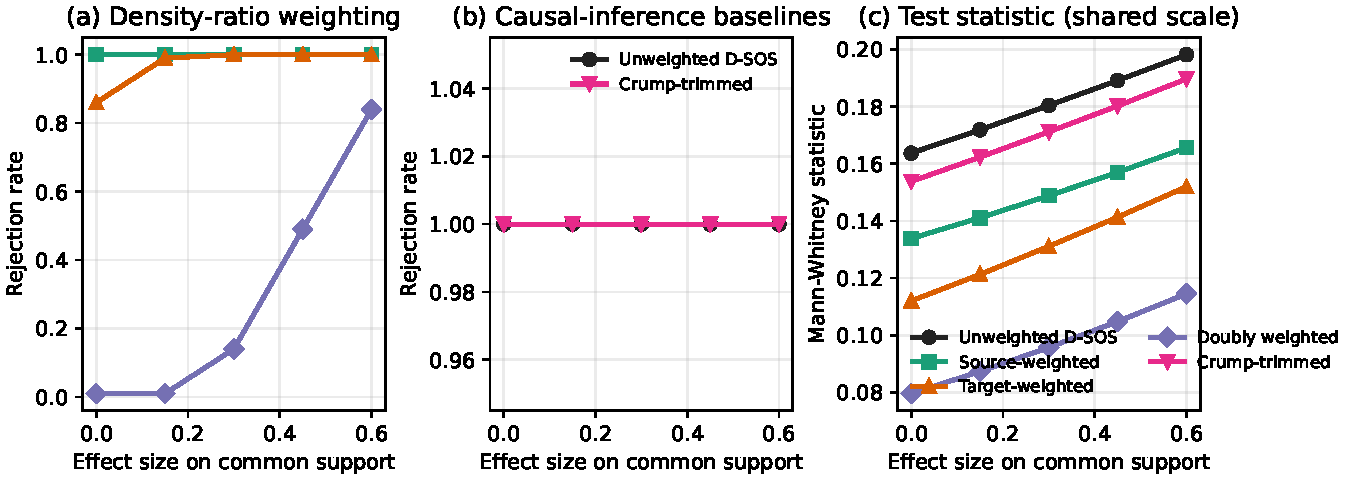
\includegraphics[width=0.98\linewidth]{figures/power_plot.pdf}
	\caption{Power for harmful shift on the common support. (a) Rejection rate for the density-ratio weighting family---unweighted, source-weighted, target-weighted, and doubly weighted. (b) Rejection rate for the causal-inference baselines---unweighted, Crump-trimmed, and overlap-weighted. (c) Mann-Whitney statistic on a common scale across all six modes, revealing the graded signal difference between weighting schemes before the binary rejection threshold. Effect size on the common support (x-axis) versus rejection rate or statistic (y-axis) across $100$ simulation repeats.}
	\label{fig:power}
\end{figure}

\subsection{Real-World Data}\label{sec:real-data-workflow}

We evaluate on four tasks from the TableShift benchmark~\cite{Gardner_2023}: HELOC (credit risk), hospital readmission, ACS income, and ACS public coverage, plus the National Supported Work (NSW) employment experiment~\cite{LaLonde_1986} as a raw-outcome example.\footnote{Three additional tasks could not be mirrored reproducibly from OpenML: PhysioNet sepsis (mirror fails checksum), College Scorecard (mirror omits Carnegie classification), and MIMIC LOS (mirror does not expose required insurance or length-of-stay columns).} For each task, we drop the split variable from the feature frame before training the source model and domain classifier, then form source-evaluation and target sets from the domain split and test three monitoring profiles: predicted risk, model confidence, and prediction error.

Figure~\ref{fig:real-data-workflow} reports $p$-values and effective sample sizes under the four weighting modes across four tasks by three profiles by four modes (48 tests). After Holm-Bonferroni correction at $\alpha = 0.05$, only HELOC predicted-risk rejections under unweighted, source-weighted, and target-weighted modes survive (all $p < 0.002$); the doubly weighted HELOC rejection disappears under common-support restriction ($p = 0.376$). No ACS or readmission test survives correction, consistent with weak-overlap contamination driving most unweighted rejections.

HELOC anchors the results. All standard modes reject for predicted risk at the permutation minimum ($p = 0.002$); with the pre-specified $\lambda = 0.5$, the doubly weighted test does not ($p = 0.376$). Effective sample size drops to $401$ ($26\%$) of $1{,}536$ source and $803$ ($29\%$) of $2{,}776$ target observations, reflecting the overlap mismatch that drives the unweighted rejection. Appendix~\ref{app:lambda} confirms this conclusion is stable across the $\lambda$ grid ($p = 0.403$ at $\lambda = 0.25$; $p = 0.312$ at $\lambda = 0.75$).

Hospital readmission shows mixed results. Risk and confidence rejections persist after common-support restriction (doubly weighted ESS: $1{,}598$ of $6{,}645$ source, $1{,}492$ of $4{,}000$ target), while the error rejection disappears under source-weighted and doubly weighted tests ($p = 0.114$). For ACS income, a single unweighted error rejection ($p = 0.046$) becomes borderline under the doubly weighted test ($p = 0.054$)---the two tests do not materially disagree (doubly weighted ESS: $2{,}321$ of $4{,}000$ source, $2{,}051$ of $4{,}000$ target). For ACS public coverage, all three profiles remain significant under every mode (doubly weighted ESS: $1{,}538$ of $4{,}000$ source, $1{,}450$ of $4{,}000$ target), consistent with harmful change affecting the common support rather than weak-overlap contamination.

The NSW employment experiment provides a complementary discrete-score setting (binary post-program earnings above \$5{,}000; PSID source $n=429$ vs.\ NSW target $n=185$; see Appendix~\ref{app:nsw}). With higher-is-better direction and no model-derived score, ties violate the continuous-distribution assumption and make the permutation test conservative. No mode rejects (unweighted $p=0.350$, doubly weighted $p=0.885$); we defer full details to the appendix and note the non-rejection likely reflects limited power under ties rather than demonstrated absence of harm.

A $\lambda$ sweep (Appendix~\ref{app:lambda}) shows the same operating-characteristic pattern: stricter common-support restriction improves specificity under mismatch while reducing effective sample size. ESS and power trade off continuously across the $\lambda$ grid; lower $\lambda$ retains specificity but concentrates weights and reduces power. A doubly weighted rejection should be interpreted together with the effective-sample-size diagnostic to balance false-alarm protection against power loss.

\subsection{Domain Classifier Sensitivity}

The method depends on domain probabilities estimated from data. We repeat the calibration experiment with logistic regression replaced by a random forest ($100$ trees, max depth $5$) and a histogram gradient-boosting classifier ($100$ iterations). Across all three classifiers, the doubly weighted test remains near nominal at every severity level (Appendix~\ref{app:domain-clf-sensitivity}).

\begin{figure}[t]
	\centering
	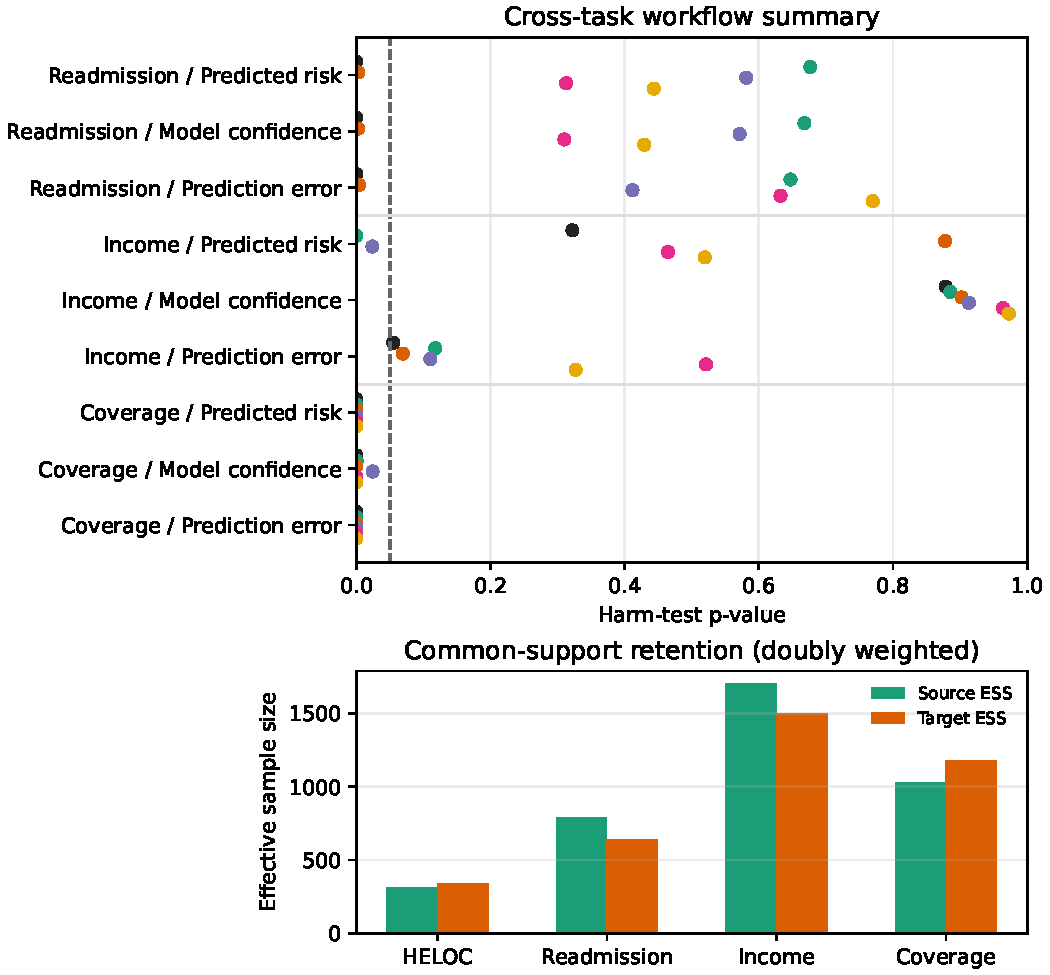
\includegraphics[width=0.98\linewidth]{figures/real_data_workflow_plot.pdf}
\caption{Real-data workflow validation. Two-panel figure: \textbf{(a)} Cross-task p-value scatter showing all tasks $\times$ workflows $\times$ modes. Each row groups the three workflows for one task; each mode is color-coded. The dashed vertical line marks the $0.05$ decision threshold. \textbf{(b)} Effective sample sizes (Kish's ESS) for source and target under the doubly weighted mode. The two bars per task show how much of each group's data survives the common-support restriction; the gap between ESS and the original sample size (not shown) diagnoses the extent of weak-overlap contamination.}
\label{fig:real-data-workflow}
\end{figure}
